\subsection{Impurities}

Diffusion of transition metals into silicon crystals result in a variety of different electrically active levels in the forbidden bandgap. Impurities is also known to create precipitates inside a silicon crystal, which change the photoluminescence spectra compared to interstitial impurities.

% 'pure' impurities
\subsubsection{Atom impurities}

Early work done by \cite{dean67} compare intrinsic silicon from the Czochralski process with doped silicon. \cite{dean67} do extensive photoluminescence study with doping atoms As, P, Sb, Bi, B, Ga, In and Al. The high intensity transverse optical lines occur at 1.0907eV, 1.0916eV, 1.0921eV, 1.0888eV, 1.0924eV, 1.0914eV, 1.0835eV and ~1.092eV respectively with the different doping atoms present. Impurities like carbon complexes with many impurities in silicon, resulting in a large variety of photoluminescence centers. Detected complexes are another C atom, one oxygen atom, one N atom, one Ga atom, the four-lithium atom complex, beryllium and numerous radiation damage centres, especially involving oxygen \cite{davies88}. See appendix \ref{energy_bands} for energies.

Doping atoms give rise to different characteristics in the photoluminescence spectra aswell. Boron doping exhibits a line right below the silicon bandgap. That particular peak is hard to detect due to a strong luminescence from the silicon itself, but its phonon replicas can be identified (figure \ref{fig:boronSiPL}). Phosphorous doping give rise to a line just below the boron line (figure \ref{fig:PSiPL}). 

Some impurities does not result in any specific photoluminescence spectra, like interstitial chromium \cite{conzelmann82}. Atleast not for wavelengths up to 1800nm. However, chromium bound with a boron atom can be identified as a peak around 0.85eV where the intensity increase linearly with laser power \cite{conzelmann82,conzelmann83}. Photoluminescence from another impurity, titanium, has been observed around 2.85eV in 4H silicon carbide by \cite{patrick74}, and in 6H by \cite{kemenade74} at 2.79eV, 2.82eV and 2.86eV named ABC lines (figure \ref{fig:Ti4HSiC}). These energies are far beyond that of the silicon bandgap, and can in cases described above, be uniquely identified.

Many of the other identified impurities are located just below the silicon bandgap in the photoluminescence spectra. Spectra for a silicon sample with a low amount of impurities can be seen in figure \ref{fig:SiPL}. Copper doping of silicon crystals results in an intense emission at 1.014eV \cite{weber82}. \cite{weronek91} study Cu doped Si and also observe a shoulder on the D1 line which presumably arises from Cu precipitates at the dislocation.

Another important impurity is iron. \cite{calao88} observe a spectrum of 0.735eV, which relate to a complex defect containing iron. Here the sample was introduced with Fe atoms into a float-zone silicon crystal (PL at figure \ref{fig:FeSiPL}). An earlier study \cite{mohring83}, observe a luminescence spectra around 1.07eV in boron-doped, iron-diffused crystalline silicon and suggest the source is Fe-B pairs. Interstitial iron Fe, is about 10 times more effective as a recombination center than Fe-B pairs by low-level lifetime measurements and therefore reduces the minority carrier diffusion length more strongly (PL at figure \ref{fig:FeBSiPL}) \cite{zoth90}.

Recent work in \cite{gundel09} show that micro-photoluminescence is an excellent tool for identifying metal precipitates in silicon as seen in figure \ref{fig:gundel_iron_precipitates}. Iron images in \cite{macdonald08} reveal internal gettering of iron to grain boundaries and dislocated regions during ingot growth. The minimum size for detection is 1$�$m, or even smaller, since the photoluminescence signal might be broadened. Precipitates from Fe and Cu are detected due to reduced band to band recombination intensity. Iron in silicon also affect the defect photoluminescence \cite{gundel09}.




% interaction with dislocations
\subsubsection{Interaction with dislocations}

Investigation in \cite{higgs92} show that transition-metal contamination plays an important role in the production of D-band luminescence from silicon samples containing either epitaxial stacking faults or oxidation-induced stacking faults. \cite{staiger94} found that Cu doping resulted in reduced intensity of D1 and D2, and the intensity of D3 and D4 become very small. \cite{weronek91} demonstrate that a complete passivation of the D-band luminescence is achieved at higher Cu and Fe concentration when deliberately contaminating high purity silicon samples which contain dislocations. However impurities like Ni, lead to no detectable changes in the spectrum \cite{weronek91}. D-band recombination in Si is found to be independent of impurities trapped at dislocations \cite{weronek91}, and \cite{sekiguchi95} concluded that metallic impurities don't seem to be related to D1 and D2 luminescence. Even so, it is still generally accepted that metal impurity influence it. Metal precipitation at crystal defects during the crystal growth can clean grains from impurities, and thus improve the performance as suggested for iron in \cite{bailey93}. A recent example of interaction with defects is iron precipitates in \cite{gundel09}, showing an enhanced defect photoluminescence at 1.3$�$m (0.95eV). The same study show that copper contamination almost completely suppress the defect photoluminescence. This is in agreement with \cite{staiger94}. Supression of defect photoluminescence by high copper concentrations was also reported in \cite{lightowlers93}. Cu precipitates can be located by  reduced intensity of the band to band photoluminescence peak, both in areas with dislocations, and without \cite{gundel09}. 

\begin{figure}%
\centering
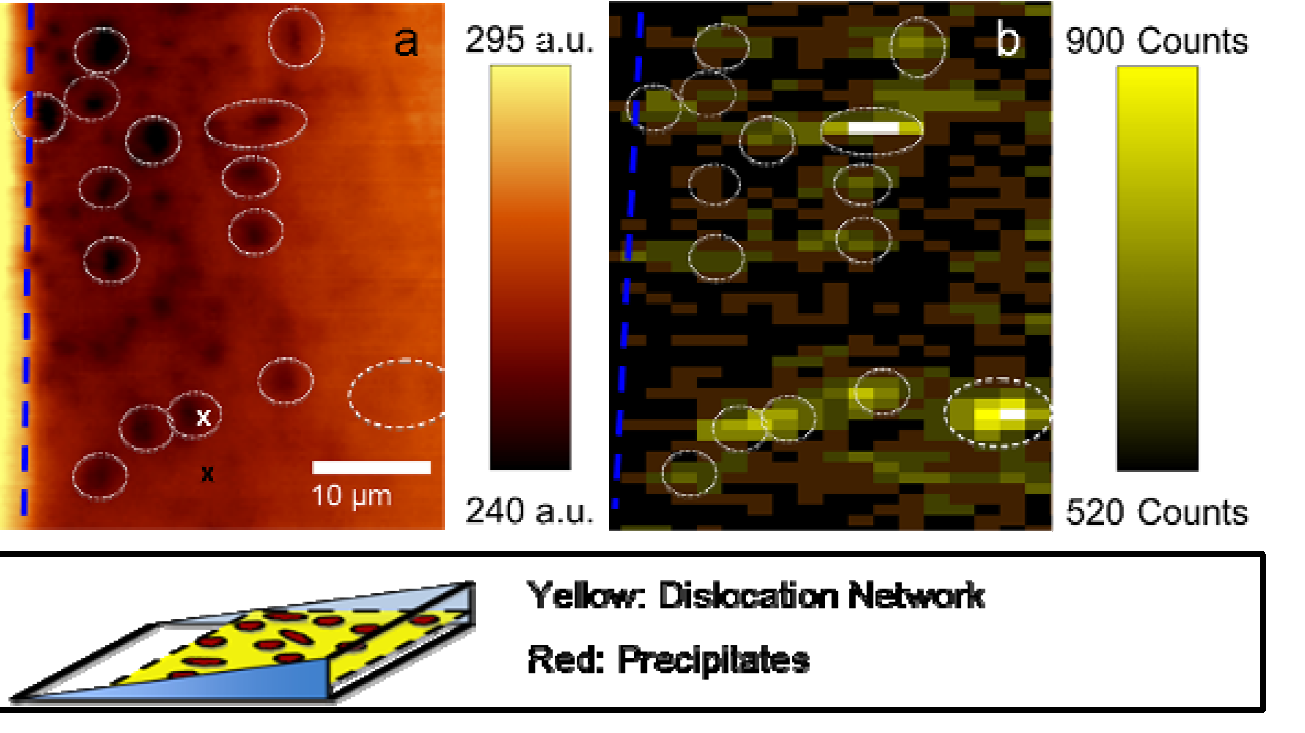
\includegraphics[width=8cm]{gundel_iron_precipitates}%
\caption[Iron precipitates]{Bottom: Scheme of the sample preparation with the polished angle. Top: A Intensity of the BB PL peak at room temperature (a), and of the iron X-ray K$\alpha$ fluorecence (b) from \cite{gundel09}. The dislocation network intersects the surface to the right of the dashed blue line. The white circles show recombination active precipitates.}
\label{fig:gundel_iron_precipitates}%
\end{figure}

Electron hole droplets (EHD), free excitons (FE) and bound excitons (BE) localized on phosphorus atoms has been steadily observed in \cite{drozdov03} with photoluminescence on samples with low-dislocated regions. When increasing dislocation density the FE, BE and EHD bands decrease sharply. This may be due exciton capture by dislocation lines D1,D2 and non-radiative recombination \cite{drozdov03}. EHD photoluminescence intensity is highly dependent on the pumping power \cite{satoshi04}. There is a linear dependence, and pumping with 3mW or less makes it hardly visible in \cite{satoshi04}.

Room temperature mapping of the 0.77eV band is attributed to oxygen precipitates in in thermally treated silicon made by the Czochralski process (Cz-Si) \cite{tajima95}. The increase of this band on the dislocation lines is due to the preferential precipitation of oxygen \cite{tajima95}.

\cite{inoue07} state that the deep-level emission from multicrystalline silicon with an intensity maximum at 0.78eV at room temperature is diffrent from that of the D1 line at low temperature. Furthermore, \cite{inoue07} suggest that the 0.78eV emission is associated with oxygen precipitation, and that the intra-grain defects are dislocation clusters decorated with oxygen impurities in addition to heavy-metal impurities. \cite{gundel08} state that the origin of trap densities in multicrystalline silicon could be structural crystal defects, which are highly decorated with oxygen precipitates.

